\documentclass{beamer}

\usepackage{beamerthemesplit}
\usepackage{graphicx}
\usepackage{subfigure}
\usepackage{amsmath,amssymb}
\usepackage{multimedia}
\usepackage{times}

\usepackage[latin1]{inputenc}
\usepackage[T1]{fontenc}
\usepackage{listings}
\usepackage{courier}
\usepackage{color}
\usepackage{rotating}

\newcommand{\re}{\text{Re}}
\newcommand{\im}{\text{Im}}
\newcommand{\de}{\mbox{d}}
\newcommand{\eref}[1]{(\ref{#1})}
\newcommand{\ii}{\text{i}}
\newcommand{\ee}{\text{e}}
\newcommand{\mathbi}[1]{\textbf{\em #1}}
\newcommand{\rem}[1]{}

% \newcommand{\heading}[1]{\centerline{\Large #1} \vspace{0.5em}}
\newcommand{\heading}[1]{\frametitle{#1}}

\newcommand{\odeint}[0]{Boost.Odeint}
\newcommand{\thrust}[0]{Thrust}
\newcommand{\vexcl}[0]{VexCL}
\newcommand{\boostcompute}[0]{Boost.Compute}
\newcommand{\viennacl}[0]{ViennaCL}
\newcommand{\cmtl}[0]{Cuda-MTL4}



% Layout specification

% \usetheme{AnnArbor}
% \usetheme{Antibes}
% \usetheme{Bergen}
% \usetheme{Berkeley}
% \usetheme{Berlin}
% \usetheme{Boadilla}
% \usetheme{boxes}
% \usetheme{CambridgeUS}
% \usetheme{Copenhagen}
% \usetheme{Darmstadt}
% \usetheme{default}
% \usetheme{Dresden}
% \usetheme{Frankfurt}
% \usetheme{Goettingen}
% \usetheme{Hannover}
% \usetheme{Ilmenau}
% \usetheme{JuanLesPins}
% \usetheme{Luebeck}
% \usetheme{Madrid}
% \usetheme{Malmoe}
% \usetheme{Marburg}
% \usetheme{Montpellier}
% \usetheme{PaloAlto}
% \usetheme{Pittsburgh}
% \usetheme{Rochester}
% \usetheme{Singapore}
% \usetheme{Szeged}
\usetheme{Warsaw}

% \usecolortheme{albatross}
% \usecolortheme{beaver}
% \usecolortheme{beetle}
% \usecolortheme{crane}
% \usecolortheme{default}
% \usecolortheme{dolphin}
% \usecolortheme{dove}
% \usecolortheme{fly}
% \usecolortheme{lily}
% \usecolortheme{orchid}
% \usecolortheme{rose}
% \usecolortheme{seagull}
% \usecolortheme{seahorse}
% \usecolortheme{sidebartab}
% \usecolortheme{structure}
% \usecolortheme{whale}
% \usecolortheme{wolverine}

% \usefonttheme{default}
% \usefonttheme{professionalfonts}
% \usefonttheme{serif}
% \usefonttheme{structurebold}
% \usefonttheme{structureitalicserif}
% \usefonttheme{structuresmallcapsserif}

% \useinnertheme{circles}
% \useinnertheme{default}
% \useinnertheme{inmargin}
% \useinnertheme{rectangles}
% \useinnertheme{rounded}

% \useoutertheme{default}
% \useoutertheme{infolines}
% \useoutertheme{miniframes}
% \useoutertheme{shadow}
% \useoutertheme{sidebar}
% \useoutertheme{smoothbars}
% \useoutertheme{smoothtree}
% \useoutertheme{split}
% \useoutertheme{tree}






% Meta

\title[Iteratorst]{Iterators and Ranges for numerical problems}
% \subtitle[Iterators]{Solving ordinary differential equations in C++}
\author[Karsten Ahnert]{Karsten Ahnert}
\institute[Ambrosys]{Ambrosys GmbH, Potsdam}
\date{\today}
%\logo{\pgfimage[width=2cm,height=2cm]{logo}}
\titlegraphic{\includegraphics[width=4cm]{ambrosys}}
\subject{Subject}
\keywords{Keyword1,Keyword2}

\newcommand{\sectionslide}[1]{\frame{\begin{centerline}{\LARGE #1}\end{centerline}}}




\definecolor{dark-gray}{gray}{0.15}
\definecolor{light-gray}{gray}{0.8}
\definecolor{lighter-gray}{gray}{0.9}

\definecolor{dark-green}{rgb}{0,0.4,0}
\definecolor{dark-red}{rgb}{0.2,0,0}

\newcommand{\highlight}[1]{\bf #1}

\lstset{
         basicstyle=\small\ttfamily, % Standardschrift
         %numbers=left,               % Ort der Zeilennummern
         numberstyle=\tiny,          % Stil der Zeilennummern
         %stepnumber=2,               % Abstand zwischen den Zeilennummern
         numbersep=0pt,              % Abstand der Nummern zum Text
         tabsize=2,                  % Groesse von Tabs
         extendedchars=true,         %
         breaklines=true,            % Zeilen werden Umgebrochen
         frame=single,         
         backgroundcolor=\color{lighter-gray},
         tabsize=2,
         keywordstyle=\color{dark-green},
         identifierstyle=,
         commentstyle=\color{dark-gray}\normalfont\rmfamily\itshape,
         stringstyle=\color{dark-red},
         showspaces=false,           % Leerzeichen anzeigen ?
         showtabs=false,             % Tabs anzeigen ?
         xleftmargin=10pt,
         xrightmargin=10pt,
         framexleftmargin=5pt,
         framexrightmargin=5pt,
         framexbottommargin=4pt,
         language=c++,
         showstringspaces=false      % Leerzeichen in Strings anzeigen ?        
 }
\lstloadlanguages{C++}


% What is shown

\beamertemplatenavigationsymbolsempty
\setbeamertemplate{footline}{}
%\setbeamertemplate{footline}{\insertframenumber}
\setbeamertemplate{headline}{}

\setbeamercolor{palette quaternary}{fg=black,bg=white}
\setbeamerfont{frametitle}{size=\Large}
\setbeamercolor{frametitle}{parent=palette quaternary}
\setbeamertemplate{frametitle}
{
  \vspace{1ex}
  \begin{beamercolorbox}[ht=2ex,wd=\paperwidth]{frametitle}
    \centerline{\insertframetitle}
  \end{beamercolorbox}
}

\parindent0pt


\begin{document}



\frame{
  \titlepage


}

\begin{frame}
  \heading{Outline}

  \tableofcontents
\end{frame}

\section{Introduction}

\sectionslide{Introduction}

\frame{
  \heading{Iterators}
  
  Unique way to traverse containers
  
  Unique way to apply iterative IO
  
  Unique way of expressing algorithms
}

\begin{frame}[fragile]{Example}
 \heading{Example -- basic use}
 \begin{lstlisting}[basicstyle=\scriptsize\ttfamily]
 for( auto iter = values.begin() ;
      iter != values.end() ;
      ++iter )
 {
     cout << *iter << endl;
 }
 \end{lstlisting}
 \pause

 \vspace{2ex}
 C++11 - use range based for
 \begin{lstlisting}[basicstyle=\scriptsize\ttfamily]
  for( auto v : values )
  {
      cout << v << endl;
  }
 \end{lstlisting}

\end{frame}



\begin{frame}[fragile]
 \heading{Example -- Container traversal}
 \begin{onlyenv}<1>
 \begin{lstlisting}
  list< double > values;
  list< double > values2( values.size() );
 \end{lstlisting}
 \end{onlyenv}
 \begin{onlyenv}<2>
 \begin{lstlisting}
  vector< double > values;
  vector< double > values2( values.size() );
 \end{lstlisting}
 \end{onlyenv} 
 \vspace{2ex}
 Can be used in
 \begin{lstlisting}
  transform( values.begin() , values.end() ,
             values2.begin() ,
             []( double x ) {
                 return x * 2.0; } );
 \end{lstlisting}
\end{frame}




\begin{frame}[fragile]
  \heading{Examples -- IO}

Input
\begin{lstlisting}[basicstyle=\scriptsize\ttfamily]
vector< double > values;  
copy_if( istream_iterator< double >( cout ) ,
         istream_iterator< double >() ,
         back_inserter( values ) ,
         []( double x ) { return x > 0.0; } );
\end{lstlisting}
\vspace{2ex}
Output
\begin{lstlisting}[basicstyle=\scriptsize\ttfamily]
vector< double > values;  
// fill values
copy_if( values.begin() , values.end() ,
         ostream_iterator< double >( std::cout , "\n" ) ,
         []( double x ) { return x > 0.0; } );
\end{lstlisting}

\end{frame}


\begin{frame}[fragile]
 \heading{Examples -- Combine algorithms}
 
 Find a nice real life example.
\end{frame}



\frame{
  \heading{Iterator types -- Concepts}
  
  \centerline{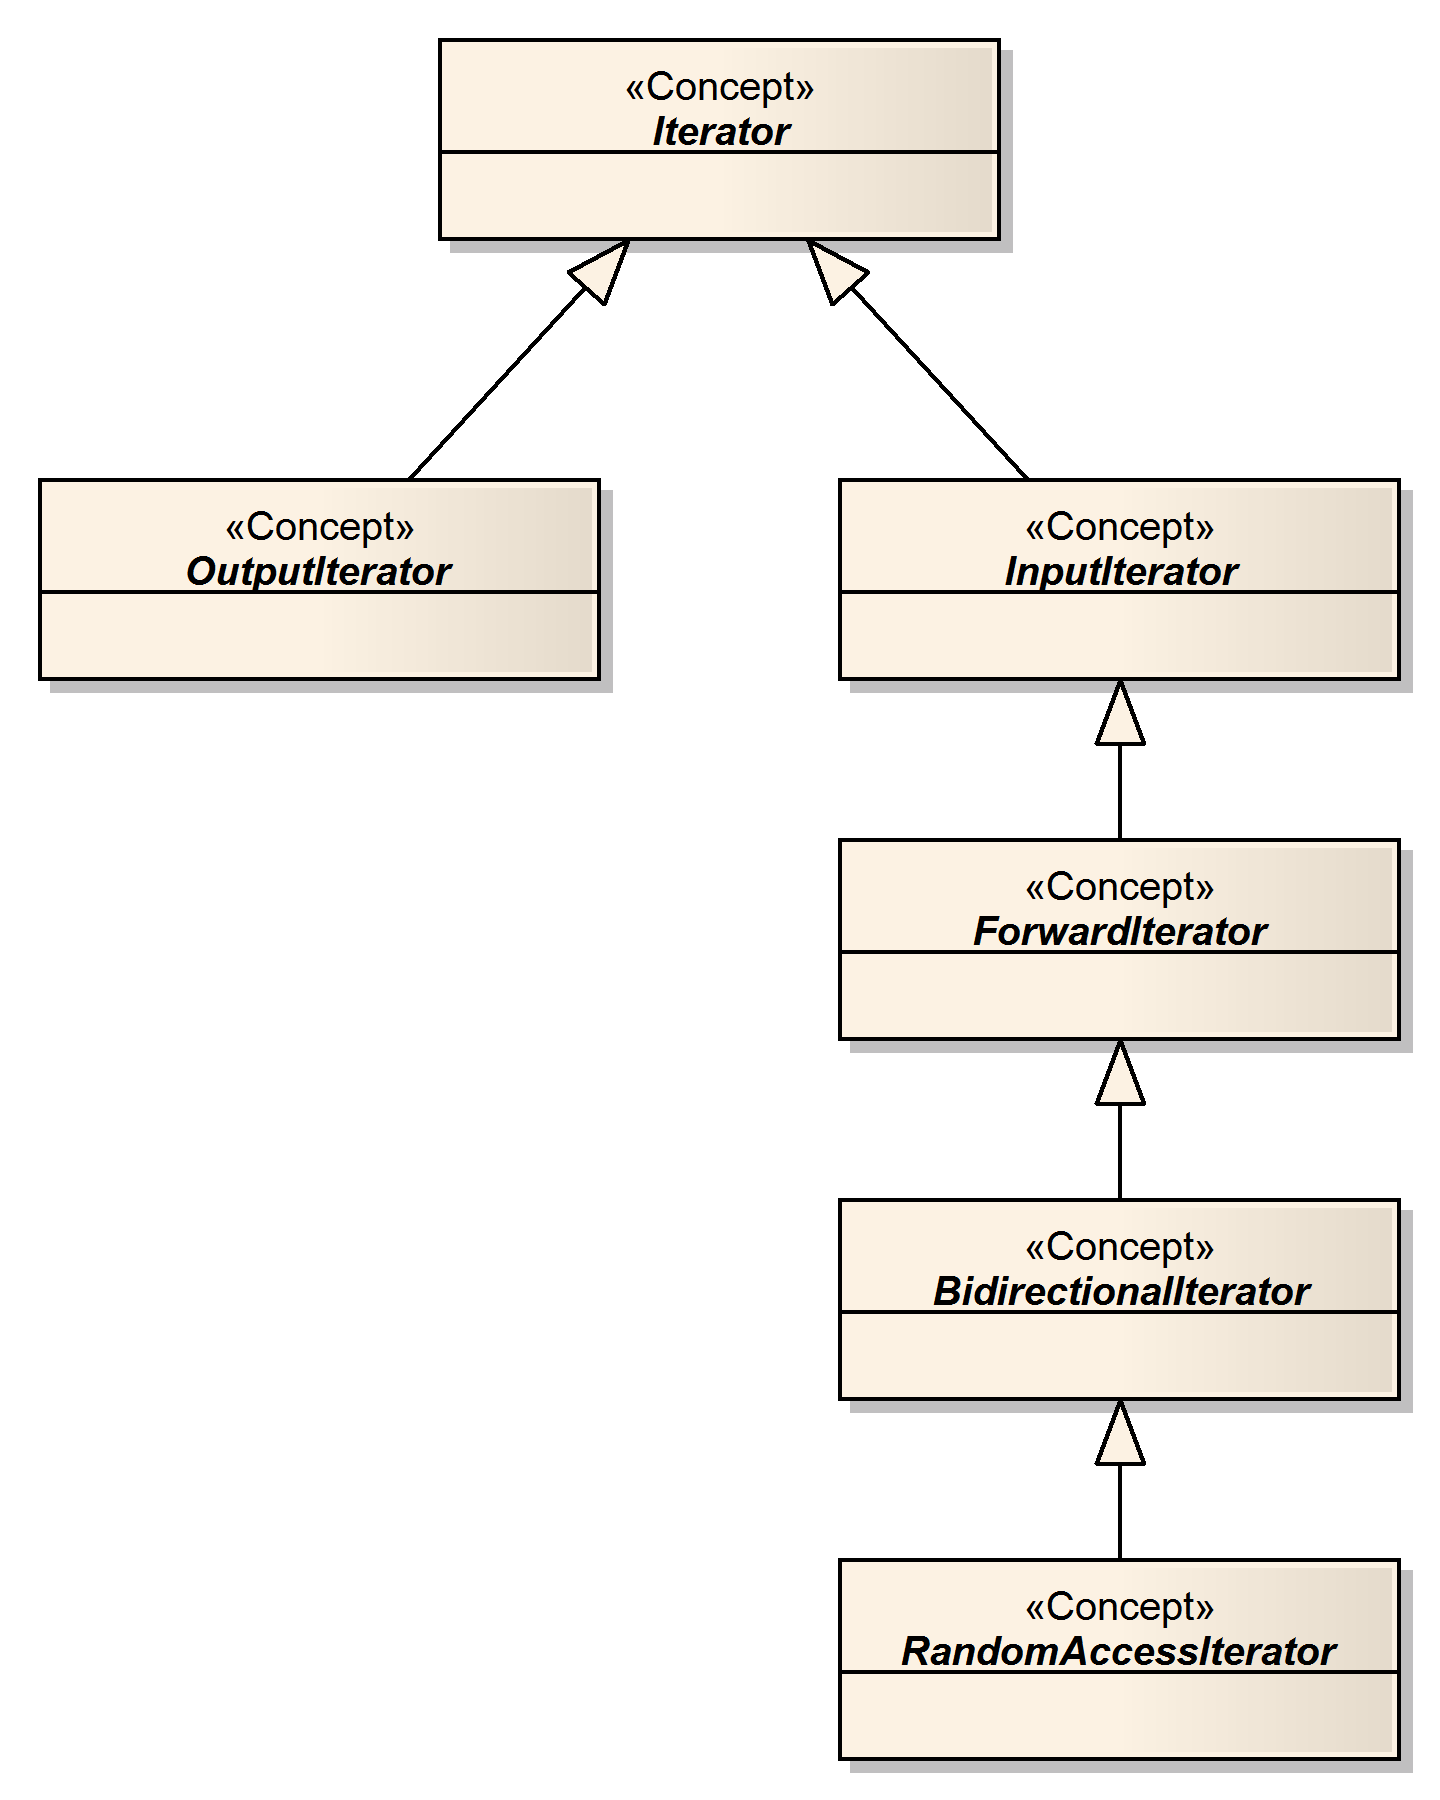
\includegraphics[width=0.5\textwidth]{IteratorsOverview}}
}

\begin{frame}[fragile]
  \heading{Iterator types -- Concepts}
  
  \vspace{2ex}
  
  \begin{columns}[T]
    \begin{column}{0.45\textwidth}
      \centerline{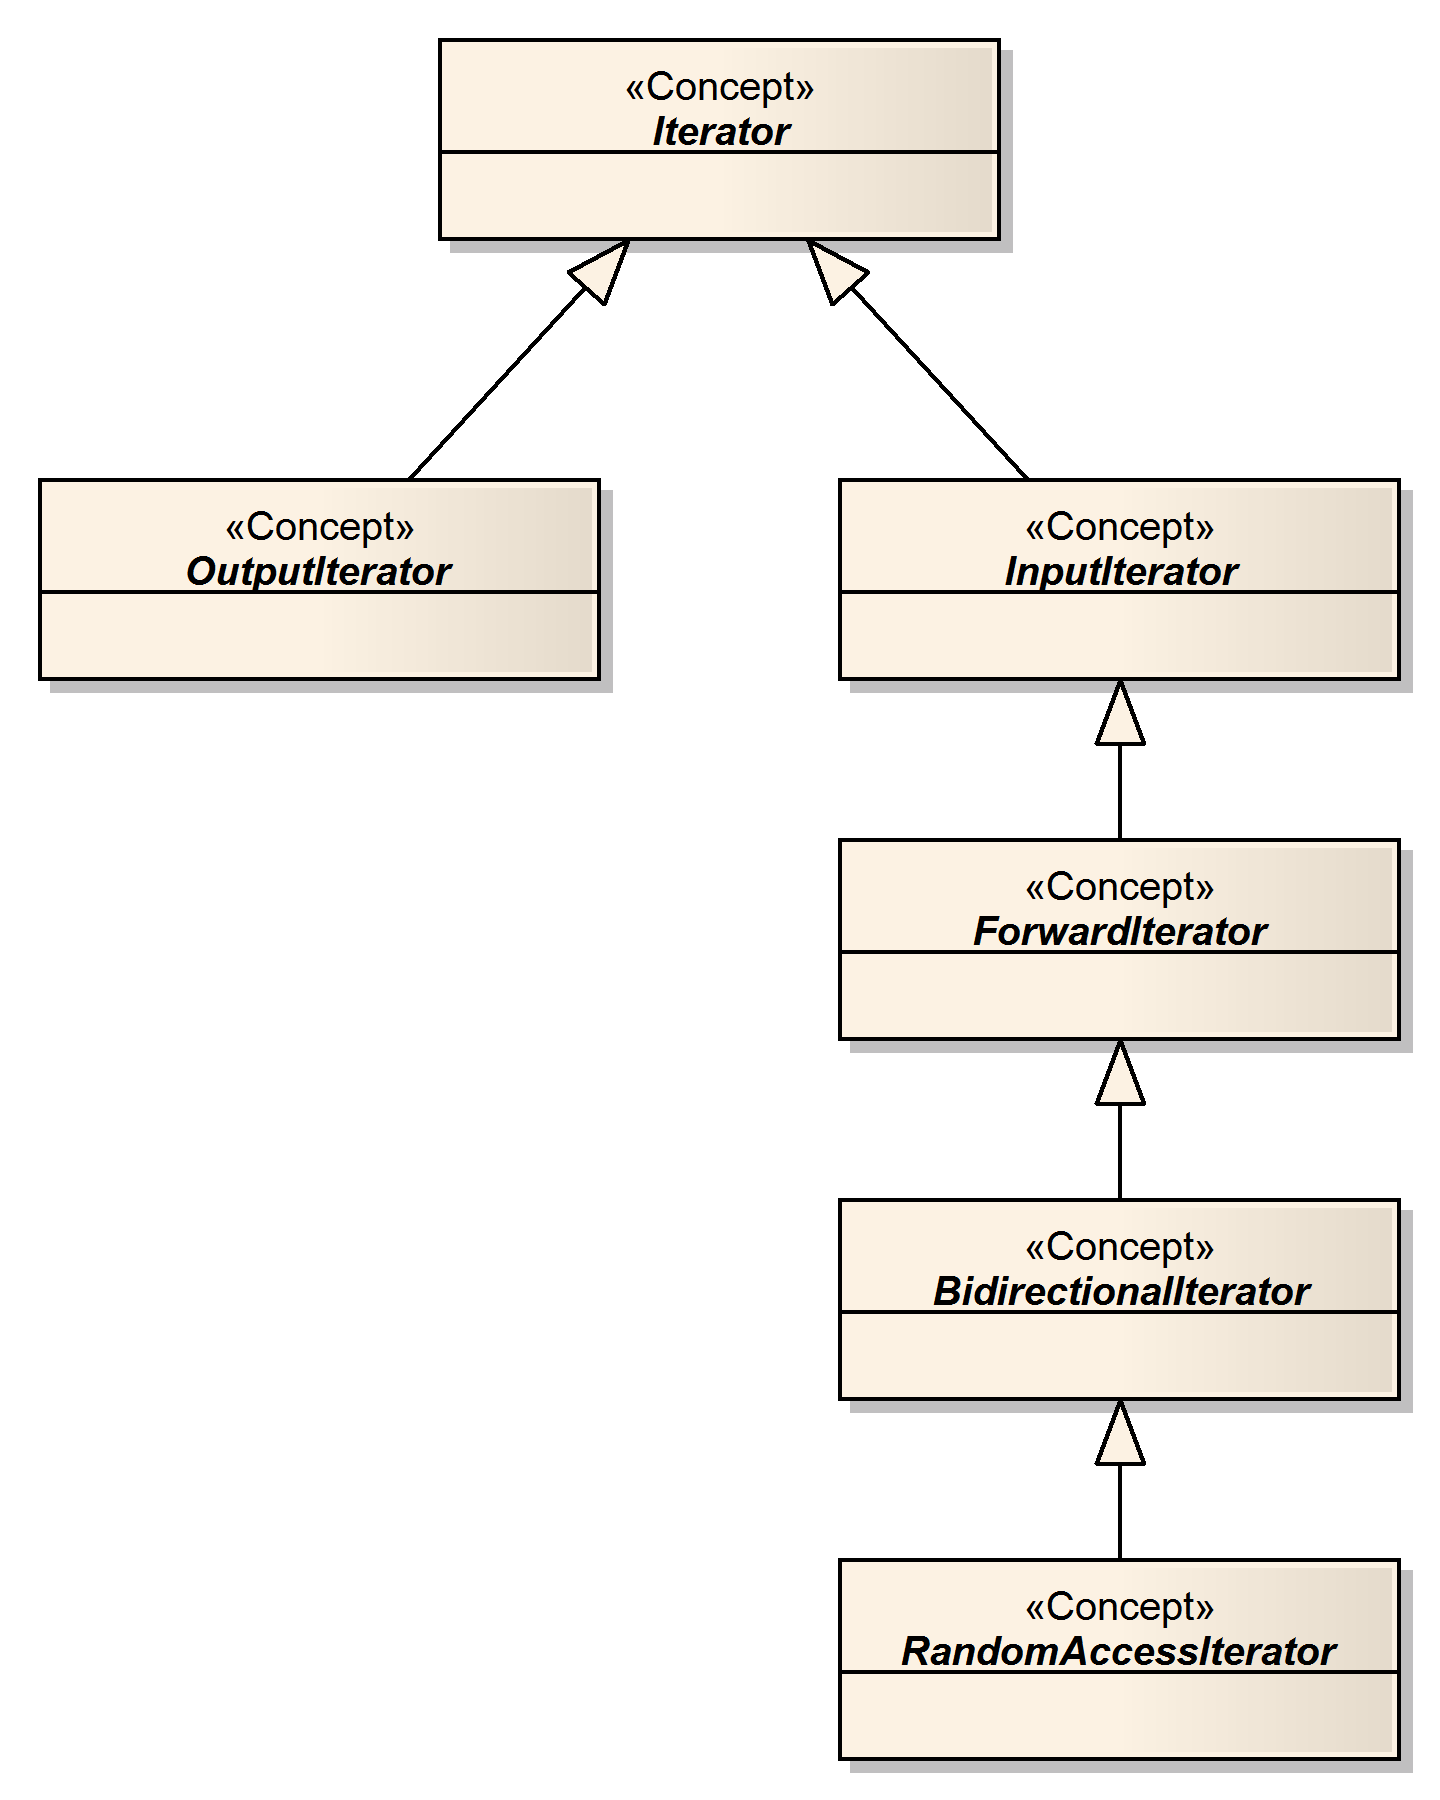
\includegraphics[width=1.0\textwidth]{IteratorsOverview}}
    \end{column}
    \begin{column}{0.55\textwidth}
      \begin{onlyenv}<1>
         OutputIterator
         
         \begin{lstlisting}
*i = o;
*i++ = o;
i++;
++i;
         \end{lstlisting}

         Are special, {\tt back\_inserter}, {\tt ostream\_iterator}, ...
      \end{onlyenv}
      \begin{onlyenv}<2>
         InputIterator a.k.a. Single-Pass Iterator
         
         \begin{lstlisting}
bool r = i != j;
val x = *i;
iterator j = ++i;
i++;
val x = *i++;
         \end{lstlisting}
{\tt istream\_iterator}, {\tt istreambuf\_iterator}

          \vspace{2ex}
          But, if {\tt i == j} then {\tt ++i != ++j}
      \end{onlyenv}
      \begin{onlyenv}<3>
         ForwardIterator
         \begin{lstlisting}
iterator j = i++;
         \end{lstlisting}

          \vspace{2ex}
          But, if {\tt i == j} then {\tt ++i == ++j}
      \end{onlyenv}
      \begin{onlyenv}<4>
         BidirectionalIterator
         \begin{lstlisting}
iterator j = --i;
iterator j = i--;
val x = *i--;
         \end{lstlisting}
         {\tt map< K , V >::iterator, list< T >::iterator}
      \end{onlyenv}
      \begin{onlyenv}<5>
         RandomAccessIterator
         \begin{lstlisting}
i += n;
i -= n;
val x = i[n];
long dist = i - j;
bool b = i < j;
         \end{lstlisting}
         {\tt vector< T >::iterator}
      \end{onlyenv}
    \end{column}
  \end{columns}
\end{frame}




\frame{
  \heading{Algorithms}
  \tiny \tt
  \begin{columns}[T]
   \begin{column}{0.2\textwidth}
      I all\_of \\
      I any\_of \\
      I none\_of \\
      I for\_each \\
      I count \\
      I count\_if \\
      I mismatch \\
      I equal \\
      I find \\
      I find\_if \\
      I find\_if\_not \\
      F find\_end \\
      I,F find\_first\_if \\
      F adjacent\_find \\
      F search \\
      F search\_n \\
      
      I,O copy \\
      I,O copy\_if \\
      I,O copy\_n \\
      B,O copy\_backward \\
      I,O move \\
      B,O move\_backward \\
      F fill \\
      F fill\_n \\
      I,O transform \\
      F generate \\
      I generate\_n \\
   \end{column}
   \begin{column}{0.2\textwidth}
      F remove \\
      F remove\_if \\
      I,O remove\_copy \\
      I,O remove\_copy\_if \\
      F replace \\
      F replace\_if \\
      I,O replace\_copy \\
      I,O replace\_copy\_if \\
      F swap\_ranges \\
      F iter\_swap \\
      B reverse \\
      B,O reverse\_copy \\
      F rotate \\
      F,O rotate\_copy \\
      R random\_shuffle \\
      R shuffle \\
      F unique \\
      I,O unique\_copy
   \end{column}
   \begin{column}{0.3\textwidth}
     is\_partitioned \\
     partition \\
     partition\_copy \\
     stable\_partition \\
     partition\_point \\
     is\_sorted \\
     is\_sorted\_until \\
     sort \\
     partial\_sort \\
     partial\_sort\_copy \\
     stable\_sort \\
     nth\_element \\
     
     lower\_bound \\
     upper\_bound \\
     binary\_search \\
     equal\_range \\
     merge \\
     inplace\_merge \\
     includes \\
     set\_difference \\
     set\_intersection \\
     set\_symmetric\_difference \\
     set\_unition 
   \end{column}
   \begin{column}{0.3\textwidth}
     is\_heap \\
     is\_heap\_until \\
     make\_heap \\
     push\_heap \\
     pop\_heap \\
     sort\_heap \\
     
     max \\
     max\_element \\
     min \\
     min\_element \\
     minmax \\
     minmax\_element \\
     lexicographical\_compare \\
     is\_permutation \\
     next\_permutation \\
     prev\_permutation \\
     iota \\
     accumulate \\
     inner\_product \\
     adjacent\_difference \\
     partial\_sum
   \end{column}
  \end{columns}


}


\begin{frame}[fragile]
  \heading{Ranges}
  
  Simplifying iterators
  
  Generalization of iterators
  
  First defined in Boost
  
  Soon in the standard library?

  \begin{lstlisting}
vector< double > values;
boost::for_each( values , []( double x ) { cout << x << endl; } );
  \end{lstlisting}


\end{frame}


\frame{
 \heading{Ranges -- more examples from boost}
 
 Filters
 
 complicated algorithms
}



\frame{
  \heading{Ranges in Boost}
  
  Ranges are pairs of iterators.
  
  Memory overhead
  
  Filters grow exponential in size
}

\frame{
  \heading{Ranges for the native C++}
  
  Introduces new concepts:
  
  Iterable, Container, Sentinel
  
  The range is the main abstraction not the iterator
  
  It holds all informations
  
  Concepts, asymmetric algorithms, sentinels have their own type.
 
}



\section{Iterators and ranges for dynamical systems}

\sectionslide{Iterators and ranges for dynamical systems}

\frame{
  \heading{Dynamical systems -- Maps}
  
  \begin{displaymath}
   x_{n+1} = f( x_n )
  \end{displaymath}
  
  \vspace{2ex}
  
  Example: Logistic map
  
  $$ x_{n+1} = r \, x_n ( 1 - x_n ) $$
  
    \centerline{ 
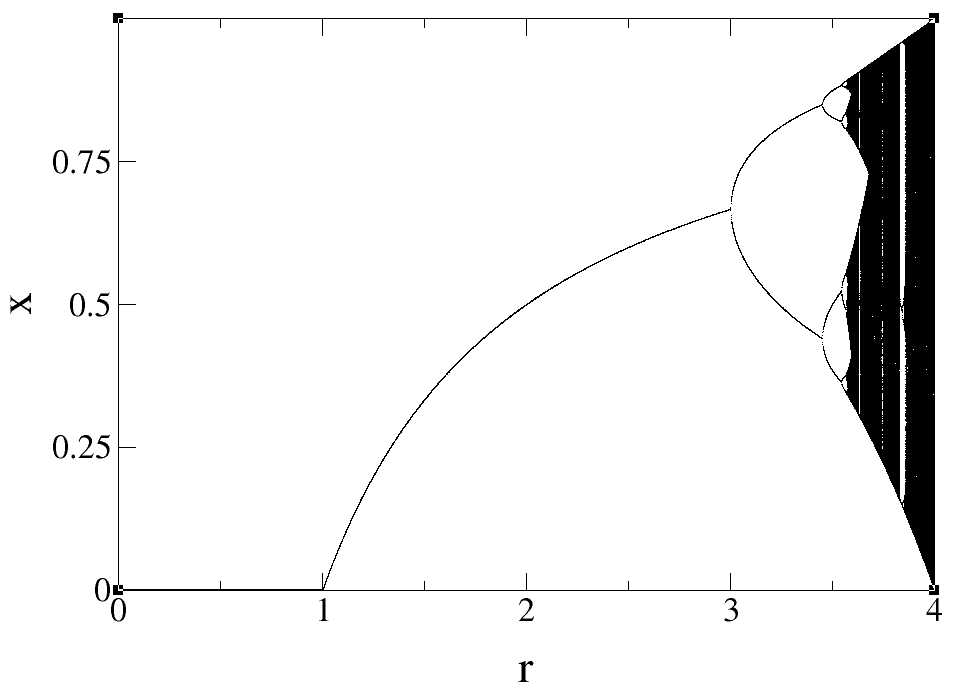
\includegraphics[draft=false,width=0.5\textwidth]{logistic_map}}
}

\frame{
  \heading{Dynamical systems -- ODEs}
  
  \begin{displaymath}
   \frac{\de x}{\de t} = f( x , t )
  \end{displaymath}
  
  \vspace{2ex}
  
  Example: Lorenz attractor
  
  $$\dot{x} = \sigma(y-x ) \quad \text{,} \quad 
\dot{y} = x ( \rho - z ) - y \quad \text{,} \quad \dot{z} = xy - \beta z$$

 \centerline{ 
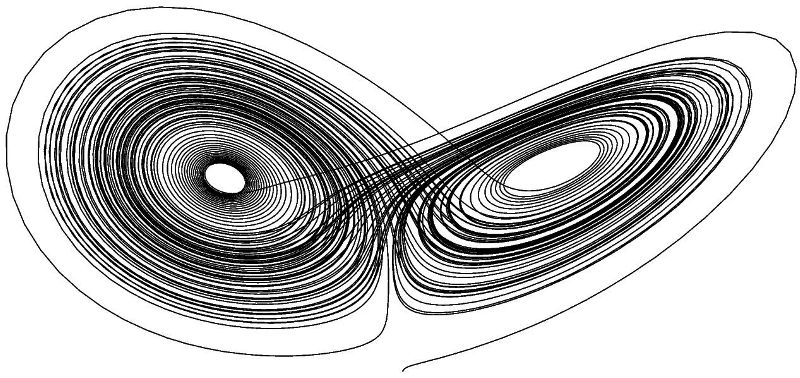
\includegraphics[draft=false,width=0.7\textwidth]{lorenz.jpg}}

  Numerical solution:
  
  $$x(t+\Delta t) = F( x(t) )$$


}

\begin{frame}[fragile]
 
  \heading{Newton method}

  Find the root
  
  $$0 = f(x)$$
  
  Newtons method
  
  \begin{itemize}
   \item Choose $x_0$
   \item Iterate $x_{n+1} = x_{n} - \frac{f(x_n)}{f'(x_n)}$
  \end{itemize}

\end{frame}


\frame{
  \heading{Map range}
  
  Abstraction for $x_{n+1} = f(x_n)$
  
  \vspace{2ex}
  
  Two versions:
  
  \begin{enumerate}
   \item {\tt map\_range} - stop predicate 
   \item {\tt counted\_map\_range} - iterates $n$-times
  \end{enumerate}
  
  Models the SinglePassRange concept
}

\frame{
  \heading{Map range - applications}
  
  \begin{itemize}
   \item Generalized iota
   \item Functional random number generators
   \item Ordinary differential equations
   \item Maps (dynamical maps)
  \end{itemize}
}

\begin{frame}[fragile]
  \heading{Map range -- implementation}
  
  \begin{lstlisting}[basicstyle=\scriptsize\ttfamily]
template< typename T1 , ... > class map_range
{
    struct iterator { ... };
 public:
    // ...
    iterator begin() { return iterator( this ); }
    iterator end() { return iterator( nullptr ); }
    // ...
};
   \end{lstlisting}
   
   Range algorithms redirect to iterator algorithms:
   \begin{lstlisting}[basicstyle=\scriptsize\ttfamily]
template< typename R , typename F >
void for_each( R const& r , F f ) {
    std::for_each( r.begin() , e.end() , f );
}
   \end{lstlisting}


\end{frame}



\begin{frame}[fragile]
  \heading{Map range}
  
\begin{lstlisting}[basicstyle=\scriptsize\ttfamily]
template< typename T , typename F , typename C >
class map_range
{
    struct iterator { ... };

  public:
    map_range( T value , F func , C condition )
    : m_value { std::move( value ) }
    , m_func { std::move( func ) }
    , m_condition( condition )
    {}
    
    iterator begin() const { return iterator( this ); }
    iterator end() const { return iterator( nullptr ); }
    
private:
    mutable T m_value;
    mutable F m_func;
    C m_condition;
};
\end{lstlisting}

\end{frame}


\begin{frame}[fragile]
  \heading{Map range}
  
\begin{lstlisting}[basicstyle=\scriptsize\ttfamily]
struct iterator {
    iterator( map_range const* _r ) : r( _r ) {}
    
    iterator& operator++() {
        r->m_value = r->m_func( r->m_value );
        if( r->m_condition( r->m_value ) ) {
            r = nullptr;
        }
        return *this;
    }
    
    T& operator*() const {
        return r->m_value; }
    bool operator==( iterator const& o ) const {
        return ( r == o.r ); }
    bool operator!=( iterator const& o ) const {
        return ! ( *this == o );
    }
    
    map_range const* r;
};
 
\end{lstlisting}

\end{frame}



\begin{frame}[fragile]
  \heading{Counted map range}
  
\begin{lstlisting}[basicstyle=\scriptsize\ttfamily]
template< typename T , typename F >
class counted_map_range
{
    struct iterator { ... };
    
public:
    counted_map_range( T value , F func , size_t max_iterations )
    : m_current_iteration { 0 }
    , m_max_iterations { max_iterations }
    , m_value { std::move( value ) }
    , m_func { std::move( func ) }
    {}
    
    iterator begin() const { return iterator( this ); }
    iterator end( void ) { return iterator( nullptr ); }
    
private:
    mutable size_t m_current_iteration = 0;
    const size_t m_max_iterations;
    mutable T m_value;
    mutable F m_func;
};
\end{lstlisting}

\end{frame}


\begin{frame}[fragile]
 \heading{Factory functions}
 
\begin{lstlisting}[basicstyle=\scriptsize\ttfamily]
template< typename T , typename F , typename C >
auto make_map_range( T t , F f , C condition )
{
    return map_range< T , F , C >(
        std::move( t ) ,
        std::move( f ) ,
        std::move( condition ) );
}
\end{lstlisting}

\begin{lstlisting}[basicstyle=\scriptsize\ttfamily]
template< typename T , typename F >
auto make_counted_map_range( T t , F f , size_t max_iterations )
{
    return counted_map_range< T , F >(
        std::move( t ) ,
        std::move( f ) , 
        max_iterations );
}
\end{lstlisting}
 


\end{frame}



\begin{frame}[fragile]
 \heading{Examples -- generalized iota}
 
 Generalized Iota:
\begin{lstlisting}[basicstyle=\scriptsize\ttfamily]
size_t n = 10;
auto iota = make_counted_map_range( 1 , []( auto x ) {
    return x * 2; } , 10 );

std::vector< int > values;
boost::copy( iota_range , std::back_inserter( values ) );
for( auto i : values ) { cout << i << endl; }
\end{lstlisting}

\end{frame}

\begin{frame}[fragile]
  \heading{Examples -- generalized iota}
  
  \textbf{Problem:} We can not easily generate a square iota:
 
  $1,4,9,16,25,36,...$
    
  \pause
 
  Introduce a projected map range.
  
  \begin{lstlisting}[basicstyle=\scriptsize\ttfamily]
auto iota_range = make_projected_counted_map_range(
    1 
    , []( auto x ) { return x+1 ; }
    , 11
    , []( auto x ) { return x*x; }
    );
for( auto i : iota_range ) { std::cout << i << std::endl; }
  \end{lstlisting}


\end{frame}

\begin{frame}[fragile]

  \heading{Example - logistic map}

\begin{lstlisting}[basicstyle=\scriptsize\ttfamily]
double r = 3.2;
auto l = [r]( auto x ) {return r * x * ( 1.0 - x ); };
auto range = make_counted_map_range( 0.5 , l , 1000 );
for( auto x : range ) { cout << x << endl; }
\end{lstlisting}
 
\end{frame}


\begin{frame}[fragile]
 \heading{Example -- Newton method}
 
\begin{lstlisting}[basicstyle=\scriptsize\ttfamily]
auto newton_range(
    auto x , auto f , auto df ,
    auto break_condition )
{
    return make_map_range(
        x ,
        [f,df]( auto x ) { return x - f( x ) / df( x ); } ,
        break_condition );
}
\end{lstlisting}

\end{frame}




\begin{frame}[fragile]
 \heading{Example -- Newton method}
 
\begin{lstlisting}[basicstyle=\scriptsize\ttfamily]
auto f = []( auto x ) { return exp(-x*x) - 0.5; };
auto df = []( auto x ) { return -2.0*x * exp(-x*x); };
auto cond  = [f]( auto x ) {
    return std::abs(f(x)) < 1.0e-12; };

auto range = newton_range( 1.0 , f , df , cond );

for( auto r : range )
    std::cout << r << " : " << f( r ) << std::endl;
\end{lstlisting}

 \centerline{ 
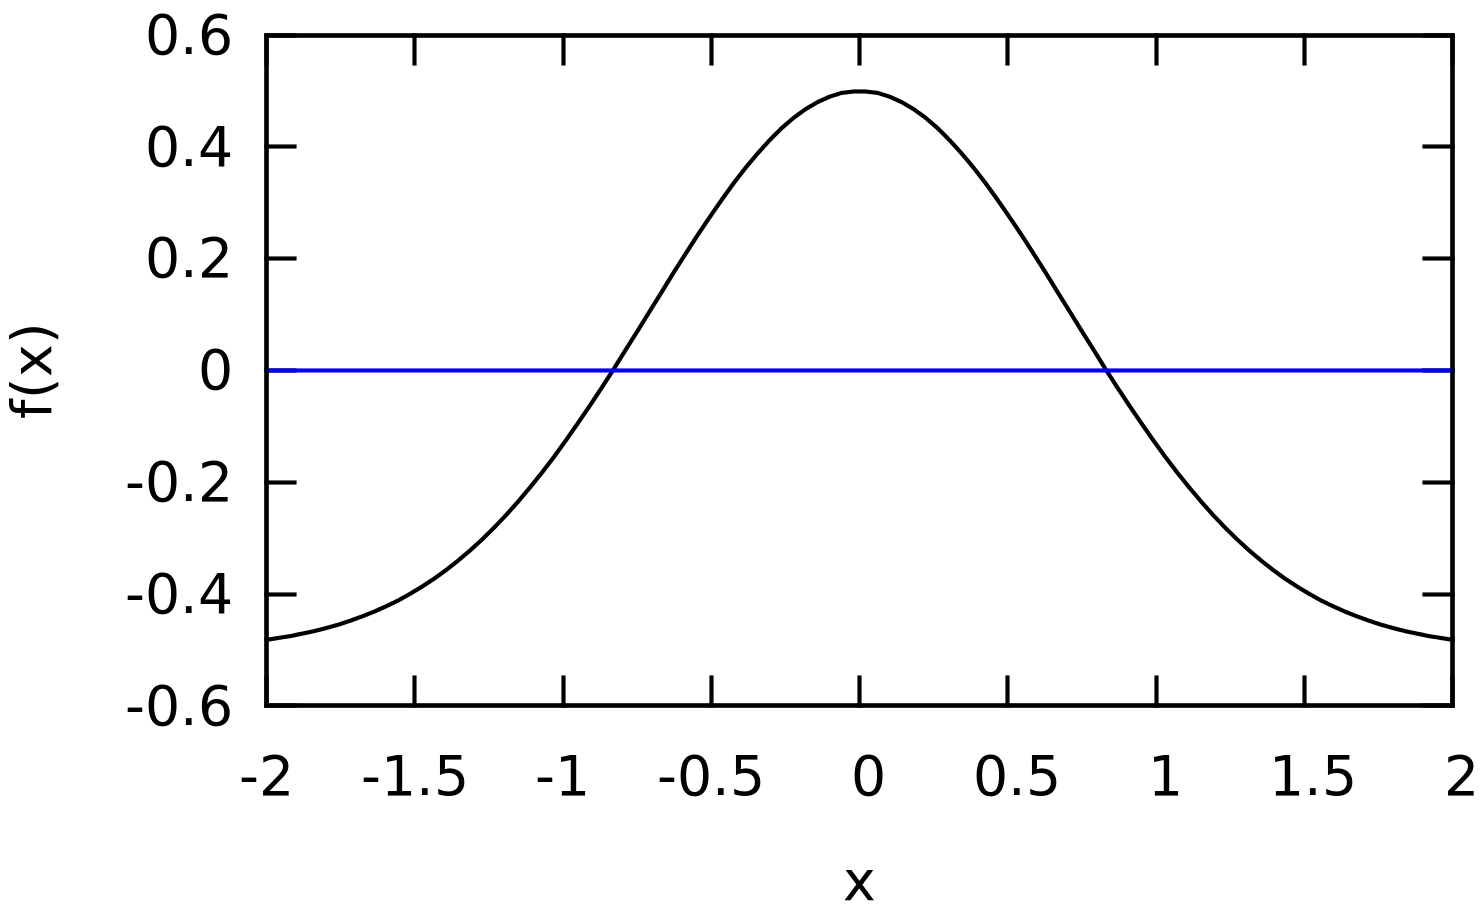
\includegraphics[draft=false,width=0.5\textwidth]{newton1}} 

\end{frame}





\begin{frame}[fragile]
  \heading{Example -- ODE solver}
  
  Solve $\dot{x} = f(x,t)$, Solver $F$ : $x(t+\delta t)=F(x(t))$
  
  Example \odeint:
  
\begin{lstlisting}[basicstyle=\tiny\ttfamily]
namespace odeint = boost::numeric::odeint;

auto lorenz = []( auto const& x , auto& dxdt , auto t )
{
    dxdt[0] = 10.0 * ( x[1] - x[0] );
    dxdt[1] = 28.0 * x[0] - x[1] - x[0] * x[2];
    dxdt[2] = -8.0 / 3.0 * x[2] + x[0] * x[1];
};

using state_type = std::array< double , 3 >;
odeint::runge_kutta4< state_type > stepper;

state_type x {{ 10.0 , 10.0 , 10.0 }};
double t = 0.0 , dt = 0.01;
stepper.do_step( lorenz , x , t , dt );
t += dt;
  \end{lstlisting}
  
Integrate functions:
\begin{lstlisting}[basicstyle=\tiny\ttfamily]
auto obs = []( auto x , auto t ) { std::cout << t << " " << x[0] << "\n"; };
odeint::integrate_const( stepper , lorenz , x , 0.0 , 10.0 , dt , obs );
\end{lstlisting}

\end{frame}

\begin{frame}[fragile]
 \heading{Example -- ODE Solver}
 
 \begin{lstlisting}[basicstyle=\tiny\ttfamily]
auto make_ode_range( auto sys , auto stepper , auto x ,
    auto t0 , auto dt , auto t1 )
{
    auto solve = [sys,stepper,dt]( auto x ) mutable { 
        stepper.do_step( sys , x.first , x.second , dt );
        x.second += dt;
        return x; };
    auto cond = [t1]( auto const& x ) { return x.second > t1; };
    auto range = make_map_range( std::make_pair(x,t0) , solver , cond );
    return range;
}
 \end{lstlisting}
 
 Can be used as
\begin{lstlisting}[basicstyle=\tiny\ttfamily]
state_type x {{ 10.0 , 10.0 , 10.0 }};
stepper_type stepper;
auto range = make_ode_range( lorenz , stepper , x , 0.0 , 0.1 , 100.0 );

for( auto r : range )
    std::cout << r.second << " " << r.first[0] << " " << r.first[1] << "\n"; 
\end{lstlisting}

\end{frame}

\begin{frame}[fragile]
 \heading{ODE ranges}
 
 Superior to integrate functions:
 \begin{itemize}
  \item Break conditions are easy
  \item ODE-Ranges can be used in a natural C++ way, {\tt find}, {\tt 
transform} , etc.
 \end{itemize}
 
 But, the implementation has some drawbacks -> custom range implementations
 \begin{itemize}
  \item Better performance.
  \item Step size control -- complicated iteration.
  \item Break condition can use the last two values.
 \end{itemize}

\end{frame}















\section{Iterators for GPUs}

\sectionslide{Iterators for GPUs algorithms}

\frame{
  \heading{High-level libraries for GPUs}
  
  \begin{enumerate}
    \item Thrust
    \item VexCL
    \item Boost.Compute
    \item ViennaCL
    \item Cuda-MTL
  \end{enumerate}
}

\frame{
  \heading{Thrust}
  
  STL-like library for Cuda
  
  Design is based on iterators
}

\frame{
  \heading{Iterators in Thrust}
  
  {\tt device\_vector::iterator}
  
  {\tt host\_vector::iterator}
  
  special iterators
  
  Algorithms
}

\frame{
  \heading{Implementation details of Thrust iterators}

}

\frame{
  \heading{Special iterators for Thrust}
  
  zip iterator
  
  transform iterator
  
}

\frame{
  \heading{Special problems - and solutions}

  Norm
}

\frame{
  \heading{Special problems - and solutions}
  
  Bucket sort
}


\frame{
  \heading{Solving an ensemble of low-dimensional ODEs}
  
  Lorenz example and ODEs
}

\section{Conclusion}

\frame{
  \heading{Conclusion}
  
  
}

\frame{
  \heading{Outlook}
}


\frame{
  \heading{References}
}


\end{document}
